\documentclass[11pt,a4paper]{article}

% ============================================================
% Packages
% ============================================================
\usepackage[utf8]{inputenc}
\usepackage[T1]{fontenc}
\usepackage[english]{babel}
\usepackage{lmodern}
\usepackage{microtype}
\usepackage{geometry}
\geometry{margin=2.5cm}
\usepackage{amsmath,amssymb,amsfonts,bm}
\usepackage{booktabs}
\usepackage{multirow}
\usepackage{subcaption}
\usepackage{float}
\usepackage{graphicx}
\graphicspath{{./}{brca_axis_figures_final/}}
\usepackage{xcolor}
\usepackage{longtable}
\usepackage{array}
\usepackage{algorithm}
\usepackage{algpseudocode}
\usepackage{tikz}
\usetikzlibrary{arrows.meta,positioning,shapes.geometric,fit,backgrounds}
\usepackage{csquotes}
\usepackage{enumitem}
\usepackage{hyperref}
\captionsetup[subfigure]{font=scriptsize}
\usepackage{makecell}
\usepackage{pdflscape}
% ============================================================
% Simple macros
% ============================================================
\newcommand{\R}{\mathbb{R}}
\newcommand{\sigmoid}{\sigma}
\newcommand{\bb}{\mathbf}
\newcommand{\softmax}{\mathrm{softmax}}

\hypersetup{
  colorlinks=true,
  linkcolor=blue,
  citecolor=blue,
  urlcolor=blue
}

\usepackage[
  backend=biber,
  style=numeric,
  sorting=none,
  sortcites=true,
  maxbibnames=999,
  natbib=true,
]{biblatex}
\addbibresource{Biblio.bib}

\title{Supplementary Material\\[0.3em]\large InterGATE: a reproducible problem-solving protocol for supervised sparse interactome learning in transcriptomic classification}
%\author{Lucía Alvarez-Frutos \and Laura Senovilla \and Alejandro Alvaro-Meca}
\date{}

\begin{document}
\maketitle

\section*{Supplementary Material}

\noindent
This supplementary document accompanies the main manuscript, \emph{InterGATE: a reproducible problem-solving protocol for supervised sparse interactome learning in transcriptomic classification}. It provides the workflow schematic, batch-correction diagnostics, additional axis-level supporting figures, detailed external-test metrics, internal backbone-replacement diagnostic results, residual enrichment figures, training pseudocode, the hyperparameter configuration used in the primary reported setting, cohort-level composition, additional biological summaries, and a description of the external supplementary data file. The self-contained software release is available at GitHub \url{https://github.com/alex241278/InterGATE}, and reproducibility data and materials are available at Zenodo \url{https://doi.org/10.5281/zenodo.20815745}.

\noindent
The supplementary material is organized as follows:
Supplementary Figure~\ref{fig:sup_combat_qc} reports ComBat batch-correction diagnostics;
Supplementary Figure~\ref{fig:sup_pipeline} provides a schematic overview of the analytical workflow;
Supplementary Figure~\ref{fig:sup_axis_boxplots} shows the axis-wise score distributions across molecular subtypes;
Supplementary Figure~\ref{fig:sup_graph_axes} shows the retained subgraph colored by biological axis;
Supplementary Algorithm~\ref{alg:sup_training} summarizes the training procedure used in the primary reported configuration;
Supplementary Table~\ref{tab:sup_cohort_by_subtype} details cohort-level sample composition;
Supplementary Table~\ref{tab:sup_combat_qc} reports quantitative ComBat harmonization diagnostics;
Supplementary Table~\ref{tab:sup_hyper} reports the hyperparameter configuration used in the primary reported setting;
Supplementary Table~\ref{tab:axes_references} summarizes the eight refined biological axes with gene composition and supporting references;
Supplementary Table~\ref{tab:sup_benchmark_full} reports the complete extended benchmark panel;
Supplementary Table~\ref{tab:sup_backbone_replacement} reports the single-seed internal backbone-replacement diagnostic;
Supplementary Table~\ref{tab:sup_test_performance} reports detailed class-specific external-test metrics;
Supplementary Table~\ref{tab:sup_confusion_matrix} reports the observed external-test confusion matrix;
Supplementary Table~\ref{tab:sup_auc_bootstrap} reports bootstrap OvR AUC estimates;
Supplementary Table~\ref{tab:sup_mean_axis_subtype} summarizes the mean axis scores by subtype;
Supplementary Table~\ref{tab:sup_residual_kegg} reports representative KEGG terms enriched in the residual gene set;
and Supplementary Data File~S1 provides the complete retained-gene list for the final consensus graph.

% ============================================================
\setcounter{figure}{0}
\renewcommand{\thefigure}{SF\arabic{figure}}
\setcounter{table}{0}
\renewcommand{\thetable}{ST\arabic{table}}
\setcounter{algorithm}{0}
\renewcommand{\thealgorithm}{SA\arabic{algorithm}}

\section*{Supplementary Figures}

\noindent
\noindent
ComBat harmonization diagnostics are shown in Supplementary Figure~\ref{fig:sup_combat_qc}. A schematic overview of the full workflow is shown in Supplementary Figure~\ref{fig:sup_pipeline}. Additional axis-wise boxplots and the axis-colored structural rendering of the retained subgraph are shown in Supplementary Figures~\ref{fig:sup_axis_boxplots} and \ref{fig:sup_graph_axes}, respectively. A stepwise training pseudocode description is provided in Supplementary Algorithm~\ref{alg:sup_training}, the full hyperparameter configuration used in the primary reported setting is summarized in Supplementary Table~\ref{tab:sup_hyper}, quantitative ComBat diagnostics are reported in Supplementary Table~\ref{tab:sup_combat_qc}, the biological axes with supporting references are listed in Supplementary Table~\ref{tab:axes_references}, the complete extended benchmark panel is reported in Supplementary Table~\ref{tab:sup_benchmark_full}, the single-seed internal backbone-replacement diagnostic is provided in Supplementary Table~\ref{tab:sup_backbone_replacement}, detailed external-test metrics are reported in Supplementary Table~\ref{tab:sup_test_performance}, the observed external-test confusion matrix is provided in Supplementary Table~\ref{tab:sup_confusion_matrix}, and bootstrap OvR AUC estimates are summarized in Supplementary Table~\ref{tab:sup_auc_bootstrap}.

\begin{figure}[!htbp]
    \centering
    \includegraphics[width=\textwidth]{FigureSF1.png}
    \caption{ComBat batch-correction diagnostics computed for the prior unsupervised inter-cohort harmonization step applied to the integrated matrix before the cohort-aware supervised partitioning.
    Quantitative silhouette scores and cross-validated classification metrics for platform, cohort, and subtype groupings are reported in Supplementary Table~\ref{tab:sup_combat_qc}.}
    \label{fig:sup_combat_qc}
\end{figure}

\clearpage

\begin{figure}[!htbp]
\centering
\resizebox{\linewidth}{!}{%
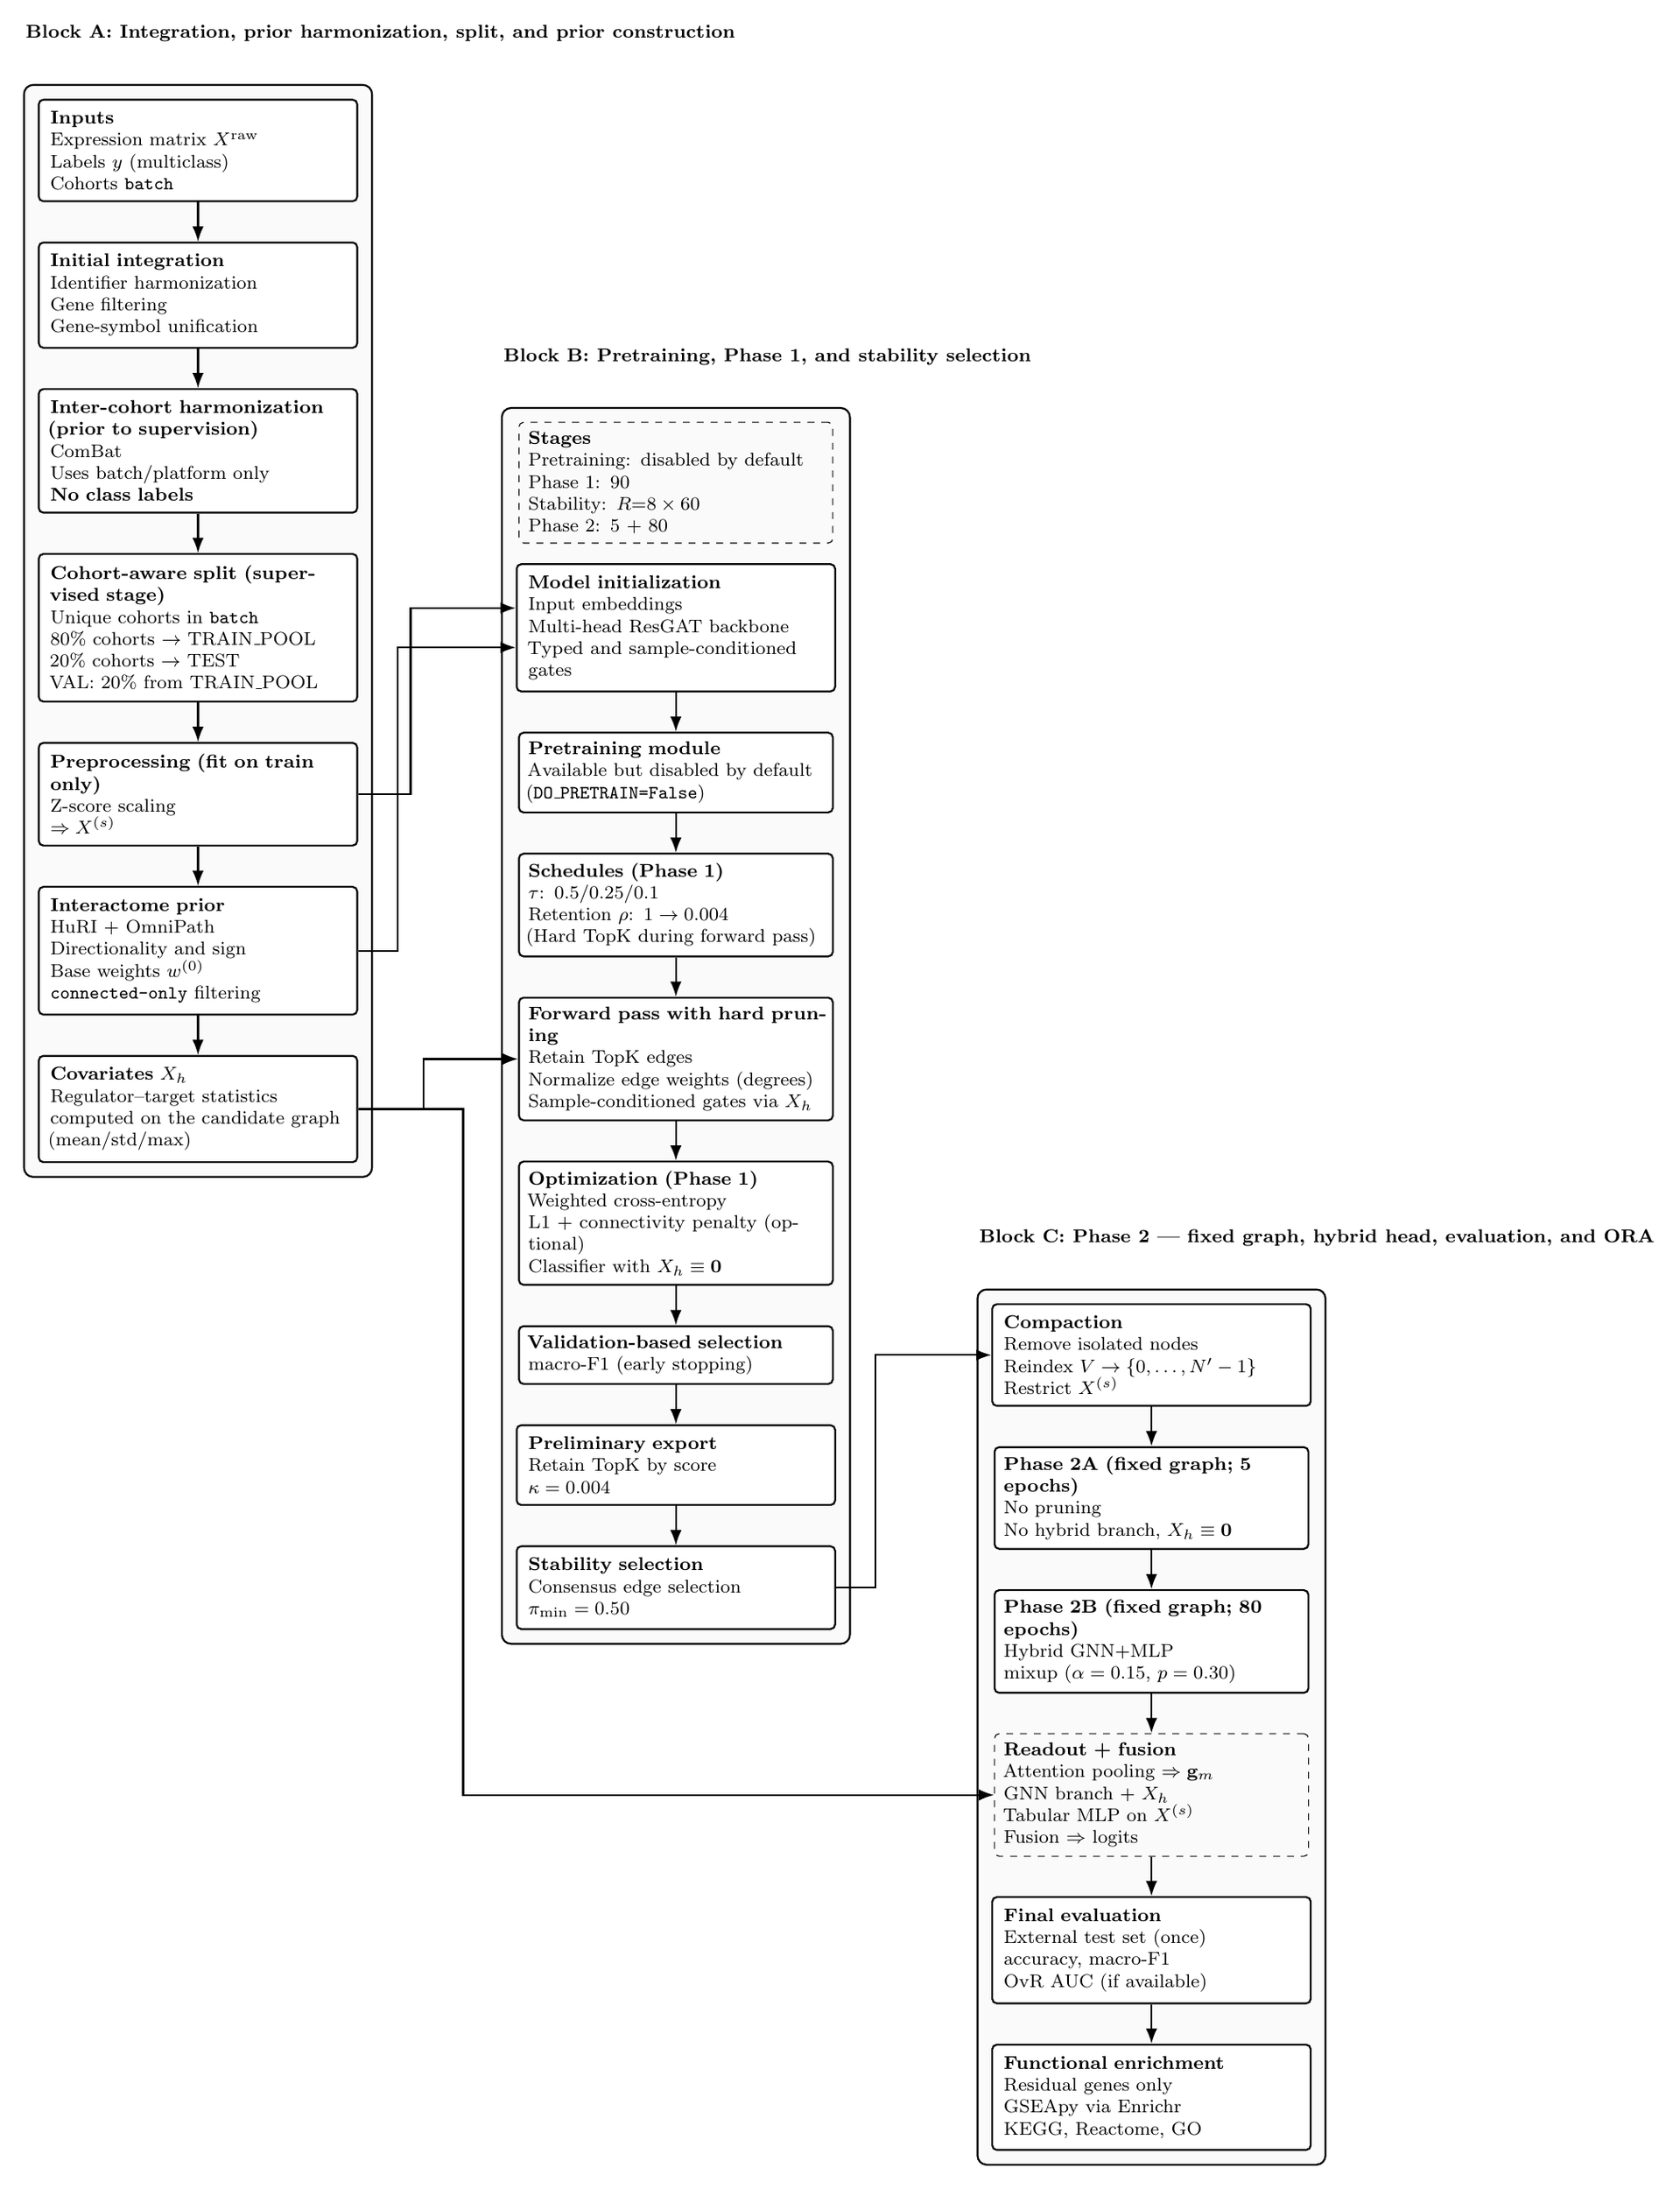
\begin{tikzpicture}[
  font=\footnotesize,
  node distance=6mm and 10mm,
  arrow/.style={-Latex, thick},
  block/.style={rectangle, rounded corners=2pt, draw, thick, fill=white,
                align=left, inner sep=5pt, text width=45mm},
  small/.style={rectangle, rounded corners=2pt, draw, thick, fill=white,
                align=left, inner sep=4pt, text width=45mm},
  group/.style={rectangle, rounded corners=4pt, draw=black, thick, fill=black!2, inner sep=6pt},
  gtitle/.style={font=\bfseries\footnotesize, anchor=south west, fill=white, inner sep=1pt},
  note/.style={rectangle, draw, dashed, rounded corners=2pt, align=left,
               inner sep=4pt, text width=45mm}
]

% Left column
\node[block] (data) { \textbf{Inputs}\\
Expression matrix $X^{\mathrm{raw}}$ \\
Labels $y$ (multiclass) \\
Cohorts \texttt{batch} };

\node[block, below=of data] (integ) { \textbf{Initial integration}\\
Identifier harmonization\\
Gene filtering\\
Gene-symbol unification };

\node[block, below=of integ] (combat) { \textbf{Inter-cohort harmonization (prior to supervision)}\\
ComBat\\
Uses batch/platform only\\
\textbf{No class labels} };

\node[block, below=of combat] (split) { \textbf{Cohort-aware split (supervised stage)}\\
Unique cohorts in \texttt{batch}\\
80\% cohorts $\to$ TRAIN\_POOL\\
20\% cohorts $\to$ TEST\\
VAL: 20\% from TRAIN\_POOL };

\node[block, below=of split] (prep) { \textbf{Preprocessing (fit on train only)}\\
Z-score scaling\\
$\Rightarrow X^{(s)}$ };

\node[block, below=of prep] (prior) { \textbf{Interactome prior}\\
HuRI + OmniPath\\
Directionality and sign\\
Base weights $w^{(0)}$\\
\texttt{connected-only} filtering };

\node[block, below=of prior] (xh) { \textbf{Covariates $X_h$}\\
Regulator--target statistics\\
computed on the candidate graph\\
(mean/std/max) };

% Center column
\node[block, right=24mm of split] (init) { \textbf{Model initialization}\\
Input embeddings\\
Multi-head ResGAT backbone\\
Typed and sample-conditioned gates };

\node[small, below=of init] (pretrain) { \textbf{Pretraining module}\\
Available but disabled by default\\
(\texttt{DO\_PRETRAIN=False}) };

\node[small, below=of pretrain] (sched) { \textbf{Schedules (Phase 1)}\\
$\tau$: 0.5/0.25/0.1\\
Retention $\rho$: $1 \to 0.004$\\
(Hard TopK during forward pass) };

\node[note, above=3mm of init] (epochs) { \textbf{Stages}\\
Pretraining: disabled by default\\
Phase 1: 90\\
Stability: $R{=}8\times 60$\\
Phase 2: 5 + 80 };

\node[small, below=of sched] (prune) { \textbf{Forward pass with hard pruning}\\
Retain TopK edges\\
Normalize edge weights (degrees)\\
Sample-conditioned gates via $X_h$ };

\node[small, below=of prune] (train1) { \textbf{Optimization (Phase 1)}\\
Weighted cross-entropy \\
L1 + connectivity penalty (optional)\\
Classifier with $X_h \equiv \mathbf{0}$ };

\node[small, below=of train1] (val1) { \textbf{Validation-based selection}\\
macro-F1 (early stopping) };

\node[block, below=of val1] (export) { \textbf{Preliminary export}\\
Retain TopK by score\\
$\kappa=0.004$ };

\node[block, below=of export] (stab) { \textbf{Stability selection}\\
Consensus edge selection\\
$\pi_{\min}=0.50$ };

% Right column
\node[block, right=24mm of val1] (compact) { \textbf{Compaction}\\
Remove isolated nodes\\
Reindex $V\to\{0,\dots,N'-1\}$\\
Restrict $X^{(s)}$ };

\node[small, below=of compact] (ftA) { \textbf{Phase 2A (fixed graph; 5 epochs)}\\
No pruning\\
No hybrid branch, $X_h\equiv\mathbf{0}$ };

\node[small, below=of ftA] (ftB) { \textbf{Phase 2B (fixed graph; 80 epochs)}\\
Hybrid GNN+MLP\\
mixup ($\alpha=0.15$, $p=0.30$) };

\node[note, below=of ftB] (readout) { \textbf{Readout + fusion}\\
Attention pooling $\Rightarrow \bb g_m$\\
GNN branch + $X_h$\\
Tabular MLP on $X^{(s)}$\\
Fusion $\Rightarrow$ logits };

\node[block, below=of readout] (test) { \textbf{Final evaluation}\\
External test set (once)\\
accuracy, macro-F1\\
OvR AUC (if available) };

\node[block, below=of test] (ora) { \textbf{Functional enrichment}\\
Residual genes only\\
GSEApy via Enrichr\\
KEGG, Reactome, GO };

% Coordinates
\path (prep.east)  ++(8mm,0) coordinate (xmain);
\path (prior.east) ++(6mm,0) coordinate (gmain);

% Arrows
\draw[arrow] (data) -- (integ);
\draw[arrow] (integ) -- (combat);
\draw[arrow] (combat) -- (split);
\draw[arrow] (split) -- (prep);
\draw[arrow] (prep) -- (prior);
\draw[arrow] (prior) -- (xh);

\draw[arrow] (prep.east) -- (xmain) |- ([yshift=3mm]init.west);
\draw[arrow] (prior.east) -- (gmain) |- ([yshift=-3mm]init.west);
\draw[arrow] (xh.east) -- ++(10mm,0) |- (prune.west);

\draw[arrow] (init) -- (pretrain);
\draw[arrow] (pretrain) -- (sched);
\draw[arrow] (sched) -- (prune);
\draw[arrow] (prune) -- (train1);
\draw[arrow] (train1) -- (val1);
\draw[arrow] (val1) -- (export);
\draw[arrow] (export) -- (stab);

\draw[arrow] (stab.east) -- ++(6mm,0) |- (compact.west);
\draw[arrow] (compact) -- (ftA);
\draw[arrow] (ftA) -- (ftB);
\draw[arrow] (ftB) -- (readout);

\draw[arrow] (xh.east) -- ++(16mm,0) |- (readout.west);

\draw[arrow] (readout) -- (test);
\draw[arrow] (test) -- (ora);

% Group boxes
\begin{pgfonlayer}{background}
  \node[group, fit=(data)(xh)] (GA) {};
  \node[group, fit=(init)(stab)(epochs)] (GB) {};
  \node[group, fit=(compact)(ora)(readout)] (GC) {};
\end{pgfonlayer}

\node[gtitle] at ([yshift=6mm]GA.north west)
  {Block A: Integration, prior harmonization, split, and prior construction};

\node[gtitle] at ([yshift=6mm]GB.north west)
  {Block B: Pretraining, Phase 1, and stability selection};

\node[gtitle] at ([yshift=6mm]GC.north west)
  {Block C: Phase 2 --- fixed graph, hybrid head, evaluation, and ORA};

\end{tikzpicture}%
}
\caption{Schematic overview of the full analytical pipeline, including data harmonization, cohort-level split, prior graph construction, graph learning with typed edge gating, stability selection, graph-fixed fine-tuning, external test evaluation, and downstream functional interpretation.}
\label{fig:sup_pipeline}
\end{figure}
\clearpage

\begin{figure}[!htbp]
    \captionsetup[subfigure]{font=footnotesize}
    \centering
    \begin{subfigure}{0.24\textwidth}
        \includegraphics[width=\linewidth]{FigureSF3A.png}
        \caption{Luminal\\Hormonal}
    \end{subfigure}
    \begin{subfigure}{0.24\textwidth}
        \includegraphics[width=\linewidth]{FigureSF3B.png}
        \caption{Cell Cycle\\Mitotic}
    \end{subfigure}
    \begin{subfigure}{0.24\textwidth}
        \includegraphics[width=\linewidth]{FigureSF3C.png}
        \caption{HER2 RTK\\MAPK}
    \end{subfigure}
    \begin{subfigure}{0.24\textwidth}
        \includegraphics[width=\linewidth]{FigureSF3D.png}
        \caption{Basal Plasticity\\TNBC}
    \end{subfigure}

    \vspace{0.5em}

    \begin{subfigure}{0.24\textwidth}
        \includegraphics[width=\linewidth]{FigureSF3E.png}
        \caption{Immune Lymphoid\\Signaling}
    \end{subfigure}
    \begin{subfigure}{0.24\textwidth}
        \includegraphics[width=\linewidth]{FigureSF3F.png}
        \caption{DNA Damage p53\\Checkpoint}
    \end{subfigure}
    \begin{subfigure}{0.24\textwidth}
        \includegraphics[width=\linewidth]{FigureSF3G.png}
        \caption{Adhesion Cytoskeleton\\Invasion}
    \end{subfigure}
    \begin{subfigure}{0.24\textwidth}
        \includegraphics[width=\linewidth]{FigureSF3H.png}
        \caption{Androgen\\Apocrine}
    \end{subfigure}
    \caption{Distribution of refined biological axis scores across molecular subtypes.}
    \label{fig:sup_axis_boxplots}
\end{figure}

\clearpage


\begin{figure}[!htbp]
    \centering
    \includegraphics[width=0.88\textwidth]{FigureSF4.png}
    \caption{Giant component of the final subgraph colored by biological axis.}
    \label{fig:sup_graph_axes}
\end{figure}


% ============================================================
\clearpage
\section*{Supplementary Algorithm}
% ============================================================

\begin{algorithm}[H]
\caption{Pretraining, supervised graph learning, stability selection, and graph-fixed fine-tuning.}
\label{alg:sup_training}
\begin{algorithmic}[1]
\State \textbf{Input:} integrated expression matrices, labels $y$, cohort vector \texttt{batch}, and prior sources (HuRI, OmniPath).
\State Harmonize identifiers, filter genes, and merge datasets into a common gene space.
\State Apply a \textbf{prior inter-cohort harmonization step} to the integrated matrix using batch/platform only and no class labels.
\State Partition the harmonized matrix into train/validation/test at the cohort level using \texttt{batch} for the subsequent supervised stage.
\State Fit post-split transformations (scaling) on train only; apply to validation and test.
\State Obtain the preprocessed matrix $X^{(s)}$.
\State Build $E$ by integrating HuRI+OmniPath (directed and signed) and apply \texttt{connected-only} filtering.
\State Build $X_h$ from regulator--target statistics on the candidate graph.
\State Initialize the backbone and gate parameters.
\vspace{1mm}

\State \textbf{Stage 0 (optional pretraining):}
\State Use training mini-batches only.
\For{epoch $=1,2,\dots,T_{\mathrm{pre}}$}
  \State Sample a mask $\mathcal{M}\subseteq V$ with probability $p_{\mathrm{mask}}$.
  \State Construct masked input $\tilde X^{(s)}$ and predict $\hat X^{(s)}$.
  \State Minimize the reconstruction loss on masked nodes.
\EndFor
\vspace{1mm}

\State \textbf{Stage 1 (supervised graph learning; validation-based selection):}
\For{epoch $=1,2,\dots,T_1$}
  \State Schedule retention fraction $\rho(\mathrm{epoch})$ (from $1$ to $0.004$) and temperature $\tau(\mathrm{epoch})$.
  \State Define the global typed and tempered score $s_e(\tau)=\theta^{\mathrm{type}}_e/\tau$.
  \State \textbf{Hard forward pruning:} retain the TopK-$\rho$ edges according to $s_e(\tau)$, yielding $E_{\mathrm{keep}}$.
  \State For each sample $m$ in the batch, compute offsets $\Delta(X_m^{\mathrm{cond}})\in\R^3$.
  \State For each retained edge $e\in E_{\mathrm{keep}}$, define the sample-conditioned score $s_{m,e}(\tau)=s_e(\tau)+\delta_{m,t_e}$.
  \State For each retained edge $e\in E_{\mathrm{keep}}$, define the soft gate $g_{m,e}(\tau)=\sigmoid\!\big(s_{m,e}(\tau)\big)$.
  \State Compute gated weights $\bar w_{m,e}(\tau)=w_e^{(0)}g_{m,e}(\tau)$ and normalize them by degree on $E_{\mathrm{keep}}$.
  \State Train for one epoch with AdamW \citep{Kingma2015Adam,Loshchilov2019AdamW} and gradient accumulation, with $X_h$ disabled in the classifier.
  \State Activate $\lambda_{\mathrm{gate}}>0$ after warm-up; optionally add $\lambda_{\mathrm{conn}}\mathcal{R}_{\mathrm{conn}}$ when connectivity regularization is enabled.
  \State Evaluate on validation (classifier without $X_h$); select by macro-F1; apply early stopping.
\EndFor
\vspace{1mm}

\State \textbf{Stage 1b (stability selection and export):}
\For{$r=1,2,\dots,R$}
  \State Reinitialize seeds (and, if applicable, weights) while keeping hyperparameters fixed.
  \State Train for $T_{\mathrm{stab}}$ epochs with the same gating/pruning scheme (without using the test set).
  \State Export $E^{(r)}_{\mathrm{final}}=\mathrm{TopK}(E,\kappa)$ according to $s_e=\theta^{\mathrm{type}}_e/\tau_{\mathrm{exp}}$, with final quota $\kappa=0.004$.
\EndFor
\State Build the consensus subgraph $E_{\mathrm{cons}}=\{e:\pi_e\ge \pi_{\min}\}$, with $\pi_{\min}=0.50$.
\State \textbf{Compact:} restrict to nodes present in $E_{\mathrm{cons}}$; reindex; trim $X^{(s)}$.
\vspace{1mm}

\State \textbf{Stage 2 (fixed graph):}
\State Build the model on the compact universe and fixed graph $E_{\mathrm{cons}}$; freeze gates and disable pruning.
\State (2A) Train for 5 epochs without the hybrid branch (\texttt{Xh=0}).
\State (2B) Train for 80 epochs with the hybrid branch and mixup (probability $p=0.30$).
\State \textbf{Test:} evaluate once on the external test set.
\end{algorithmic}
\end{algorithm}

% ============================================================
\clearpage
\section*{Supplementary Tables}
% ============================================================

\begin{table}[!htbp]
\centering
\caption{Cohort-by-subtype sample composition of the final integrated breast cancer resource used in the study.}
\label{tab:sup_cohort_by_subtype}
\resizebox{\textwidth}{!}{%
\begin{tabular}{lrrrrrr}
\toprule
\textbf{Cohort} & \textbf{HER2} & \textbf{LumA} & \textbf{LumB} & \textbf{Normal} & \textbf{TNBC} & \textbf{Total} \\
\midrule
GSE1456   & 15  & 39   & 23  & 0   & 25  & 102 \\
GSE15852  & 0   & 0    & 0   & 43  & 0   & 43 \\
GSE162228 & 22  & 54   & 40  & 0   & 17  & 133 \\
GSE19615  & 14  & 0    & 0   & 0   & 28  & 42 \\
GSE20711  & 26  & 13   & 22  & 2   & 27  & 90 \\
GSE21653  & 24  & 89   & 49  & 29  & 75  & 266 \\
GSE25066  & 37  & 160  & 78  & 44  & 189 & 508 \\
GSE32646  & 18  & 0    & 0   & 0   & 26  & 44 \\
GSE58812  & 0   & 0    & 0   & 0   & 107 & 107 \\
GSE65194  & 39  & 29   & 30  & 11  & 55  & 164 \\
GSE96058  & 348 & 1709 & 767 & 225 & 360 & 3409 \\
TCGA      & 59  & 421  & 193 & 114 & 117 & 904 \\
\midrule
\textbf{Total} & \textbf{602} & \textbf{2514} & \textbf{1202} & \textbf{468} & \textbf{1026} & \textbf{5812} \\
\bottomrule
\end{tabular}%
}
\end{table}


\begin{table}[!htbp]
\centering
\caption{Quantitative diagnostics of the prior unsupervised ComBat harmonization step, based on 20-component PCA embeddings before and after correction. For each grouping variable, silhouette scores assess clustering structure, and macro-F1 values correspond to 5-fold cross-validated $k$-nearest-neighbour prediction from PCA embeddings. Large decreases in platform- and cohort-related metrics indicate suppression of technical structure, whereas retention of subtype-related metrics supports preservation of biologically relevant signal.}
\label{tab:sup_combat_qc}
\resizebox{\textwidth}{!}{%
\begin{tabular}{lrrrrrr}
\toprule
\textbf{Grouping} & \textbf{Silhouette before} & \textbf{Silhouette after} & \(\Delta\) \textbf{silhouette} & \textbf{kNN macro-F1 before} & \textbf{kNN macro-F1 after} & \(\Delta\) \textbf{macro-F1} \\
\midrule
Platform & 0.378 & -0.081 & -0.459 & 1.000 & 0.441 & -0.559 \\
Cohort   & 0.679 & -0.160 & -0.839 & 1.000 & 0.106 & -0.894 \\
Subtype  & -0.050 & 0.062 & +0.112 & 0.815 & 0.760 & -0.055 \\
\bottomrule
\end{tabular}%
}
\end{table}

\begin{table}[!htbp]
\centering
\caption{Hyperparameters and configuration used in the primary reported setting.}
\label{tab:sup_hyper}
\begin{tabular}{@{}p{0.23\linewidth}p{0.73\linewidth}@{}}
\toprule
\textbf{Block} & \textbf{Main parameters} \\
\midrule
Preprocessing &
Gene-wise scaling fitted on train only; the primary reported configuration used \texttt{StandardScaler} (\texttt{SCALE\_MODE=standard}). \\

Cohort-aware split &
Applied \textbf{after} the unsupervised inter-cohort harmonization step. Unique cohorts are enumerated and randomly split at the cohort level, with 80\% assigned to \emph{train\_pool} and 20\% to the external test set (\texttt{train\_size=0.80}, \texttt{random\_state=1234}); validation is obtained by simple random sampling from \emph{train\_pool} with fraction \texttt{VAL\_SIZE=0.20}. \\

Candidate graph $E$ &
Directed integration of HuRI (physical PPI) and OmniPath (signaling). Edge types $t\in\{0,1,2\}$: HuRI, OmniPath$(+)$, OmniPath$(-)$. \texttt{connected-only} filtering removes isolated genes after prior construction. \\

Typed gating &
Global logit $\theta_e$ and type-specific calibration: $\theta^{\mathrm{type}}_e=a_{t_e}\theta_e+b_{t_e}$, with learnable $a_t,b_t$. \\

Sample-conditioned gating &
In the primary configuration, the sample-dependent offset acts on the pre-sigmoid score:
$s_e(\tau)=\theta^{\mathrm{type}}_e/\tau$,
$s_{m,e}(\tau)=s_e(\tau)+\delta_{m,t_e}$,
with $\Delta:\R^F\to\R^{3}$ (lightweight MLP on $X_h$). Some ablation variants use a global offset instead. \\

ResGAT backbone &
Hidden dimension $H=64$, $L=3$ ResGAT blocks, $K=4$ heads, dropout 0.10, ELU/GELU activations depending on block, LayerNorm, and residual connections. \\

Global pooling &
Multi-head attention pooling with $P=4$ heads. \\

Pretraining &
Disabled in the GitHub default/paper-aligned configuration (\texttt{DO\_PRETRAIN=False}). The masked gene-modeling module remains available in the code as an optional pretraining stage. \\

Graph learning (Phase 1) &
$T_1=90$ epochs; temperature schedule \texttt{gate\_tau}: 0.5 (epochs 1--10), 0.25 (11--20), 0.1 (21+); hard retention $\rho$ decreases exponentially to \texttt{KEEP\_MIN=0.004}. AdamW \citep{Kingma2015Adam,Loshchilov2019AdamW} with learning rate $2\times10^{-3}$, gradient accumulation (\texttt{ACCUM\_STEPS=8}), batch size 20, and patience 30. \\

Regularization &
Sparsity: per-edge L1 penalty (\texttt{EDGE\_L1\_PER\_EDGE=1e-5}). In the selected primary configuration (\texttt{FULL}), connectivity regularization is enabled in the GitHub default, using \texttt{CONNECTIVITY\_LAMBDA=0.002} and threshold \texttt{CONNECTIVITY\_MIN\_DEG=0.05} (\texttt{ADD\_CONNECTIVITY\_PENALTY=True}; \texttt{CONNECTIVITY\_USE\_ABS=True}). Alternative ablation variants selectively disabled or modified this component. \\

Stability selection &
$R=8$ runs (\texttt{STAB\_RUNS=8}), $T_{\mathrm{stab}}=60$ epochs, final quota $\kappa=0.004$ (\texttt{STAB\_KEEP\_FINAL}), consensus threshold $\pi_{\min}=0.50$ (\texttt{STAB\_FREQ\_THR}). \\

Fine-tuning (Phase 2) &
(2A) $T_{2A}=5$ epochs with fixed graph and \emph{without} the hybrid branch (and without $X_h$ in the classifier); (2B) $T_{2B}=80$ epochs with fixed graph, hybrid branch enabled, and mixup (\texttt{MIXUP\_ALPHA=0.15}, \texttt{MIXUP\_P=0.30}). In the main hybrid configuration: \texttt{USE\_HYBRID\_MODEL=True}, \texttt{HYBRID\_TAB\_LAYERS=2}, \texttt{HYBRID\_TAB\_DROPOUT=0.20}, \texttt{HYBRID\_FUSION\_DROPOUT=0.20}, \texttt{HYBRID\_BLEND\_LOGITS=False}. The parameter \texttt{HYBRID\_BLEND\_INIT=0.70} remains available in the code but is only relevant when \texttt{HYBRID\_BLEND\_LOGITS=True}. \\

Model selection &
Phase 1: macro-F1-based validation selection with early stopping and patience 30. Phase 2: best-checkpoint selection again uses validation macro-F1 on the fixed consensus graph. The default GitHub configuration serializes the final run with \texttt{FINAL\_SELECT\_METRIC=macro\_f1} and \texttt{RUN\_FINAL\_AFTER\_ABLATION=True}. \\
\bottomrule
\end{tabular}
\end{table}


% ============================================================
% TABLE: Refined biological axes with gene composition and references
% ============================================================



\begin{table}[!htbp]
\centering
\caption{Summary of the eight refined biological axes derived from the 291-gene consensus graph. Each axis groups genes with established roles in the corresponding biological program. The gene lists were manually curated from the retained graph signature based on prior functional knowledge. Representative references supporting the biological coherence of each axis are provided.}
\label{tab:axes_references}
\resizebox{\textwidth}{!}{%
\begin{tabular}{lcccl}
\toprule
\textbf{Biological axis} & \textbf{$n$} & \textbf{Representative genes} & \textbf{Shared} & \textbf{References} \\
\midrule
Luminal Hormonal & 8 &
  \makecell[cl]{\texttt{ESR1}, \texttt{PGR}, \texttt{GATA3}, \texttt{GREB1},\\
               \texttt{ESR2}, \texttt{PHLDA1}, \texttt{LRIG1}, \texttt{RXRA}} &
  -- & \citet{Perou2000MolecularPortraits,Sorlie2003BreastSubtypes,Parker2009PAM50} \\
\addlinespace
Cell Cycle Mitotic & 14 &
  \makecell[cl]{\texttt{AURKA}, \texttt{AURKB}, \texttt{BUB1}, \texttt{CDC7}, \texttt{CDC23}, \texttt{CDCA3}, \texttt{CDK1},\\
               \texttt{CDK2}, \texttt{CEP55}, \texttt{E2F1}, \texttt{FOXM1}, \texttt{PLK1}, \texttt{TTK}, \texttt{ZWINT}} &
  -- & \citet{Whitfield2002CellCycle,Desmedt2008Proliferation} \\
\addlinespace
HER2 RTK MAPK & 14 &
  \makecell[cl]{\texttt{ERBB2}, \texttt{EGFR}, \texttt{IGF1R}, \texttt{MET}, \texttt{PDGFRB}, \texttt{AKT1}, \texttt{MAP2K1},\\
               \texttt{MAP2K2}, \texttt{MAPK1}, \texttt{MAPK3}, \texttt{MAPK14}, \texttt{PLCG1}, \texttt{SRC}, \texttt{LYN}} &
  \texttt{EGFR} & \citet{Slamon1987HER2,TCGA2012BRCA,Dhillon2007MAPK} \\
\addlinespace
Basal Plasticity TNBC & 8 &
  \makecell[cl]{\texttt{KRT6A}, \texttt{KRT16}, \texttt{SOX10}, \texttt{VGLL1},\\
               \texttt{VGLL3}, \texttt{EGFR}, \texttt{EMP1}, \texttt{MSLN}} &
  \texttt{EGFR}, \texttt{MSLN} & \citet{Perou2000MolecularPortraits,Nielsen2004BasalLike,Lehmann2011TNBC} \\
\addlinespace
Immune Lymphoid Signaling & 14 &
  \makecell[cl]{\texttt{CD79A}, \texttt{CXCL9}, \texttt{DEF6}, \texttt{GRAP2}, \texttt{HCK}, \texttt{JAK3}, \texttt{ITPKB},\\
               \texttt{PAX5}, \texttt{SYK}, \texttt{S1PR1}, \texttt{SOCS1}, \texttt{TRAF1}, \texttt{TRAF2}, \texttt{ZBP1}} &
  -- & \citet{Denkert2018TILs,Tokunaga2018CXCL9} \\
\addlinespace
DNA Damage p53 Checkpoint & 11 &
  \makecell[cl]{\texttt{ATM}, \texttt{ERCC3}, \texttt{FANCG}, \texttt{KAT5}, \texttt{PRKDC}, \texttt{TP53},\\
               \texttt{MDM2}, \texttt{PTEN}, \texttt{DAPK1}, \texttt{STK11}, \texttt{SIRT1}} &
  -- & \citet{TCGA2012BRCA,Shiloh2003ATM,DAndrea2003Fanconi} \\
\addlinespace
Adhesion Cytoskeleton Invasion & 12 &
  \makecell[cl]{\texttt{ABI2}, \texttt{FLNA}, \texttt{ITGB1}, \texttt{ITGB1BP1}, \texttt{MMP2}, \texttt{PTK2},\\
               \texttt{RHOA}, \texttt{ROCK1}, \texttt{LASP1}, \texttt{NCK1}, \texttt{NCK2}, \texttt{SDCBP}} &
  -- & \citet{Desgrosellier2010Integrins,Sahai2002RhoGTPases} \\
\addlinespace
Androgen Apocrine & 2 &
  \texttt{AR}, \texttt{MSLN} &
  \texttt{MSLN} & \citet{Farmer2005Apocrine,Lehmann2011TNBC} \\
\midrule
\multicolumn{2}{l}{\textit{Total unique genes: 81}} & \multicolumn{3}{l}{\textit{Total assignments: 83 (\texttt{EGFR} and \texttt{MSLN} appear in two axes each)}} \\
\bottomrule
\end{tabular}%
}
\end{table}


% ============================================================
% Complete extended benchmark panel
% ============================================================
\begin{table}[!htbp]
\centering
\caption{Complete extended benchmark panel under the same cohort-aware split. This table includes the full set of tabular, signature-restricted, fixed-prior, and rewired-prior models mentioned in the main benchmark panel. The internal backbone-replacement diagnostic is reported separately in Supplementary Table~\ref{tab:sup_backbone_replacement}.}
\label{tab:sup_benchmark_full}
\resizebox{\textwidth}{!}{%
\begin{tabular}{llcccc}
\toprule
\textbf{Family} & \textbf{Model} & \textbf{Validation macro-F1} & \textbf{Test accuracy} & \textbf{Test macro-F1} & \textbf{Test OvR macro-AUC} \\
\midrule
Proposed graph-learning
& \texttt{FULL} & 0.928 & 0.948 & 0.924 & 0.991 \\
\midrule
\multirow{8}{*}{Full-expression tabular}
& \texttt{catboost} & 0.964 & 0.892 & 0.896 & 0.984 \\
& \texttt{extratrees} & 0.860 & 0.910 & 0.894 & 0.986 \\
& \texttt{random\_forest} & 0.938 & 0.918 & 0.902 & 0.983 \\
& \texttt{elasticnet\_logreg} & 0.862 & 0.889 & 0.870 & 0.987 \\
& \texttt{linear\_svm\_calibrated} & 0.850 & 0.851 & 0.832 & 0.974 \\
& \texttt{mlp\_graph\_free} & 0.829 & 0.839 & 0.801 & 0.976 \\
& \texttt{xgboost} & 0.975 & 0.848 & 0.837 & 0.971 \\
& \texttt{lightgbm} & 0.965 & 0.891 & 0.890 & 0.982 \\
\midrule
\multirow{4}{*}{291-gene signature tabular}
& \texttt{random\_forest\_291} & 0.943 & 0.942 & 0.900 & 0.990 \\
& \texttt{xgboost\_291} & 0.953 & 0.912 & 0.893 & 0.985 \\
& \texttt{elasticnet\_logreg\_291} & 0.787 & 0.865 & 0.844 & 0.981 \\
& \texttt{mlp\_graph\_free\_291} & 0.822 & 0.806 & 0.842 & 0.973 \\
\midrule
\multirow{4}{*}{Graph controls}
& \texttt{fixed\_prior\_gnn} & 0.792 & 0.845 & 0.827 & 0.977 \\
& \texttt{fixed\_prior\_hybrid} & 0.845 & 0.848 & 0.827 & 0.972 \\
& \texttt{rewired\_prior\_gnn} & 0.770 & 0.867 & 0.846 & 0.984 \\
& \texttt{rewired\_prior\_hybrid} & 0.851 & 0.864 & 0.843 & 0.973 \\
\bottomrule
\end{tabular}%
}
\end{table}

\begin{table}[!htbp]
\centering
\caption{Internal backbone-replacement diagnostic under the FULL InterGATE protocol. All variants used the same cohort-aware split, hidden dimension 64, three message-passing layers, four attention/pooling heads where applicable, final edge quota 0.004, and the hybrid head enabled. Only the message-passing backbone was changed. The analysis used seed 1 only, so the table is interpreted as an architectural diagnostic rather than as a replacement for the full stability-selected 291-gene consensus model.}
\label{tab:sup_backbone_replacement}
\resizebox{\textwidth}{!}{%
\begin{tabular}{llcccccccc}
\toprule
\textbf{Configuration} & \textbf{Backbone} & \textbf{Seed} & \textbf{Phase-1 val macro-F1} & \textbf{Final edges} & \textbf{Compact genes} & \textbf{Test accuracy} & \textbf{Test macro-F1} & \textbf{Test weighted-F1} & \textbf{Test OvR macro-AUC} \\
\midrule
\texttt{FULL\_GAT} & GAT/ResGAT & 1 & 0.864 & 205 & 264 & 0.925 & 0.924 & 0.927 & 0.993 \\
\texttt{FULL\_GRAPH\_TRANSFORMER} & GraphTransformer & 1 & 0.686 & 205 & 304 & 0.857 & 0.841 & 0.862 & 0.976 \\
\texttt{FULL\_GIN} & GIN & 1 & 0.682 & 205 & 343 & 0.857 & 0.834 & 0.862 & 0.973 \\
\texttt{FULL\_GRAPHSAGE} & GraphSAGE & 1 & 0.708 & 205 & 271 & 0.848 & 0.830 & 0.851 & 0.974 \\
\bottomrule
\end{tabular}%
}
\end{table}



\begin{table}[!htbp]
\centering
\caption{Classification performance on the external test set (\(n=1{,}055\)). Point estimates and 95\% bootstrap confidence intervals are shown for class-specific and global metrics.}
\label{tab:sup_test_performance}
\resizebox{\textwidth}{!}{%
\begin{tabular}{lccccccc}
\toprule
\textbf{Class / Metric} & \textbf{Support} & \textbf{Precision} & \textbf{95\% CI} & \textbf{Recall} & \textbf{95\% CI} & \textbf{F1} & \textbf{95\% CI} \\
\midrule
HER2   & 77  & 0.855 & [0.772, 0.928] & 0.844 & [0.758, 0.922] & 0.850 & [0.785, 0.905] \\
LumA   & 421 & 0.955 & [0.934, 0.973] & 1.000 & [1.000, 1.000] & 0.977 & [0.966, 0.986] \\
LumB   & 193 & 0.995 & [0.983, 1.000] & 0.969 & [0.942, 0.990] & 0.982 & [0.966, 0.994] \\
Normal & 114 & 0.885 & [0.825, 0.941] & 0.877 & [0.812, 0.934] & 0.881 & [0.833, 0.923] \\
TNBC   & 250 & 0.958 & [0.930, 0.982] & 0.908 & [0.872, 0.942] & 0.932 & [0.908, 0.954] \\
\midrule
Macro avg    & 1055 & 0.929 & [0.908, 0.949] & 0.920 & [0.897, 0.941] & 0.924 & [0.903, 0.943] \\
Weighted avg & 1055 & 0.948 & [0.934, 0.961] & 0.948 & [0.935, 0.960] & 0.947 & [0.934, 0.960] \\
\bottomrule
\end{tabular}%
}
\end{table}


\begin{table}[!htbp]
\centering
\caption{Observed confusion matrix on the external test set. Rows correspond to true labels and columns to predicted labels.}
\label{tab:sup_confusion_matrix}
\begin{tabular}{lccccc}
\toprule
\textbf{True class} & \textbf{HER2} & \textbf{LumA} & \textbf{LumB} & \textbf{Normal} & \textbf{TNBC} \\
\midrule
HER2   & 65 & 1 & 1 & 1 & 9 \\
LumA   & 0 & 421 & 0 & 0 & 0 \\
LumB   & 3 & 3 & 187 & 0 & 0 \\
Normal & 0 & 13 & 0 & 100 & 1 \\
TNBC   & 8 & 3 & 0 & 12 & 227 \\
\bottomrule
\end{tabular}
\end{table}

\begin{table}[!htbp]
\centering
\caption{One-vs-rest AUC on the external test set. Point estimates and 95\% bootstrap confidence intervals are shown for each class and for the macro-average.}
\label{tab:sup_auc_bootstrap}
\begin{tabular}{lcc}
\toprule
\textbf{Class / Metric} & \textbf{OvR AUC} & \textbf{95\% CI} \\
\midrule
HER2      & 0.977 & [0.956, 0.993] \\
LumA      & 0.999 & [0.998, 1.000] \\
LumB      & 0.999 & [0.997, 1.000] \\
Normal    & 0.991 & [0.985, 0.996] \\
TNBC      & 0.992 & [0.987, 0.996] \\
\midrule
Macro avg & 0.991 & [0.987, 0.996] \\
\bottomrule
\end{tabular}
\end{table}





\begin{landscape}
\begin{table}[!htbp]
\centering
\caption{Mean biological axis scores by molecular subtype. Positive values indicate relative activation with respect to the full cohort mean.}
\label{tab:sup_mean_axis_subtype}
\begin{tabular}{lrrrrrrrr}
\toprule
\textbf{Subtype} & \textbf{Lum.–Horm.} & \textbf{Cell Cycle} & \textbf{HER2–RTK} & \textbf{Basal–TNBC} & \textbf{Immune} & \textbf{DNA Dam.–p53} & \textbf{Adhes.–Inv.} & \textbf{Andro.–Apoc.} \\
\midrule
Normal &  0.159 & $-$0.956 &  0.129 &  0.593 &  0.117 & $-$0.020 &  0.205 &  0.002 \\
LumA   &  0.338 & $-$0.481 & $-$0.039 & $-$0.126 & $-$0.154 &  0.015 & $-$0.025 &  0.084 \\
LumB   &  0.141 &  0.508 & $-$0.091 & $-$0.604 & $-$0.147 &  0.040 & $-$0.204 & $-$0.027 \\
HER2   & $-$0.498 &  0.410 &  0.136 & $-$0.027 &  0.201 & $-$0.155 & $-$0.007 &  0.030 \\
TNBC   & $-$0.774 &  0.779 &  0.065 &  0.763 &  0.377 &  0.017 &  0.210 & $-$0.192 \\
\bottomrule
\end{tabular}
\end{table}
\end{landscape}

\begin{table}[!htbp]
\centering
\caption{Representative KEGG terms enriched in the 210 residual genes not assigned to curated axes.}
\label{tab:sup_residual_kegg}
\begin{tabular}{p{5.8cm}ccr}
\toprule
\textbf{KEGG term} & \textbf{Overlap} & \textbf{Adj. \emph{P}} & \textbf{Odds ratio} \\
\midrule
MAPK signaling pathway & 24/294 & $1.33\times10^{-11}$ & 8.37 \\
Pathways in cancer & 31/531 & $1.33\times10^{-11}$ & 5.97 \\
Lipid and atherosclerosis & 19/215 & $5.63\times10^{-10}$ & 8.95 \\
Wnt signaling pathway & 16/166 & $4.38\times10^{-9}$ & 9.73 \\
Neurotrophin signaling pathway & 13/119 & $4.63\times10^{-8}$ & 11.06 \\
ErbB signaling pathway & 11/85 & $1.25\times10^{-7}$ & 13.31 \\
HIF-1 signaling pathway & 11/109 & $1.15\times10^{-6}$ & 10.04 \\
Insulin signaling pathway & 12/137 & $1.15\times10^{-6}$ & 8.61 \\
Chemokine signaling pathway & 13/192 & $4.33\times10^{-6}$ & 6.53 \\
\bottomrule
\end{tabular}
\end{table}

%\begin{table}[!htbp]
%\centering
%\caption{Structural summary of the axis-colored giant component of the final retained graph. Node counts in this table refer only to the visible nodes assigned to each biological axis within the giant component shown in Supplementary Figure~\ref{fig:sup_graph_axes}; they do not represent the full number of axis-assigned genes in the complete 291-gene retained signature.}
%\label{tab:sup_graph_axis_hubs}
%\begin{tabular}{lcl}
%\toprule
%\textbf{Visible module} & \textbf{$n$ nodes} & \textbf{Representative hubs} \\
%\midrule
%Luminal Hormonal & 8 & \texttt{ESR1}, \texttt{RXRA}, \texttt{ESR2}, \texttt{GATA3}, \texttt{GREB1}, \texttt{LRIG1}, \texttt{PGR}, \texttt{PHLDA1} \\
%Cell Cycle Mitotic & 14 & \texttt{CDK1}, \texttt{FOXM1}, \texttt{AURKA}, \texttt{CEP55}, %\texttt{E2F1}, \texttt{TTK}, \texttt{AURKB}, \texttt{BUB1}, \texttt{CDC23}, \texttt{CDC7}, \texttt{CDCA3}, \texttt{CDK2}, \texttt{PLK1}, \texttt{ZWINT} \\
%HER2 RTK MAPK & 14 & \texttt{EGFR}, \texttt{LYN}, \texttt{MAPK1}, \texttt{MAPK14}, \texttt{MAPK3}, \texttt{ERBB2}, \texttt{IGF1R}, \texttt{AKT1}, \texttt{MAP2K1}, \texttt{MAP2K2}, \texttt{MET}, \texttt{PDGFRB}, \texttt{PLCG1}, \texttt{SRC} \\
%Basal Plasticity TNBC & 7 & \texttt{KRT16}, \texttt{EMP1}, \texttt{KRT6A}, \texttt{MSLN}, \texttt{SOX10}, \texttt{VGLL1}, \texttt{VGLL3} \\
%Immune Lymphoid Signaling & 14 & \texttt{CD79A}, \texttt{SYK}, \texttt{TRAF1}, \texttt{CXCL9}, \texttt{DEF6}, \texttt{GRAP2}, \texttt{HCK}, \texttt{ITPKB}, \texttt{JAK3}, \texttt{PAX5}, \texttt{S1PR1}, \texttt{SOCS1}, \texttt{TRAF2}, \texttt{ZBP1} \\
%DNA Damage p53 Checkpoint & 11 & \texttt{TP53}, \texttt{MDM2}, \texttt{ATM}, \texttt{DAPK1}, \texttt{ERCC3}, \texttt{FANCG}, \texttt{KAT5}, \texttt{PRKDC}, \texttt{PTEN}, \texttt{SIRT1}, \texttt{STK11} \\
%Adhesion Cytoskeleton Invasion & 12 & \texttt{PTK2}, \texttt{LASP1}, \texttt{NCK2}, \texttt{RHOA}, \texttt{ROCK1}, \texttt{SDCBP}, \texttt{ABI2}, \texttt{FLNA}, \texttt{ITGB1}, \texttt{ITGB1BP1}, \texttt{MMP2}, \texttt{NCK1} \\
%Androgen Apocrine & 1 & \texttt{AR} \\
%\bottomrule
%\end{tabular}
%\end{table}



%La tabla ST11$ describe qué se ve en la visualización del grafo (la componente gigante): no todos los 81 genes del eje aparecen conectados entre sí en esa componente, así que los recuentos son menores (6 de 8 luminales, 1 de 2 andrógenos, etc.) y los "representative hubs" son los nodos con más aristas dentro de esa subred visible.
%La tabla ST4 es la definición completa de los ejes: los 81 genes asignados, con referencias bibliográficas que justifican la curación. La relación es jerárquica: la  tabla ST4 define los ejes a nivel biológico (qué genes y por qué), y la  tabla ST11 muestra cómo esos mismos ejes se manifiestan topológicamente dentro de la componente gigante del grafo retenido. Los genes que faltan en la primera tabla (p. ej. GREB1, RXRA en Luminal, o MSLN en Androgen) simplemente no forman parte de esa componente conexa — están en el grafo completo de 291 genes pero quedan aislados o en componentes menores.

% ============================================================
\clearpage
\section*{Supplementary External Data File}
% ============================================================

\noindent
To keep the main manuscript concise while preserving direct reproducibility of the final learned signature, the retained-gene universe is provided as a single external supplementary file.

\noindent\textbf{Supplementary Data File~S1: Final retained graph genes.}
This file contains the complete list of genes retained in the final consensus graph, together with graph-related identifiers and node-level structural information exported from the final retained network.

\printbibliography[heading=none]

\end{document}
